%!TEX root = ../main.tex

\chapter{Results\label{chap:results}}

The approach presented in the previous section was applied on a prerecorded rosbag from a real-world experiment.
Four \ac{UAV}s were used in this experiment.
The mapped area was $50 \times 35$ meters with $0.4$ m resolution.
The experiment took approximately 8 minutes and 250 cones were measured.

The results are presented in figure \ref{fig:A} and \ref{fig:B}. 
\begin{figure}[!h]
  \centering
  \subfloat[True positions of sources (MBq)] {
    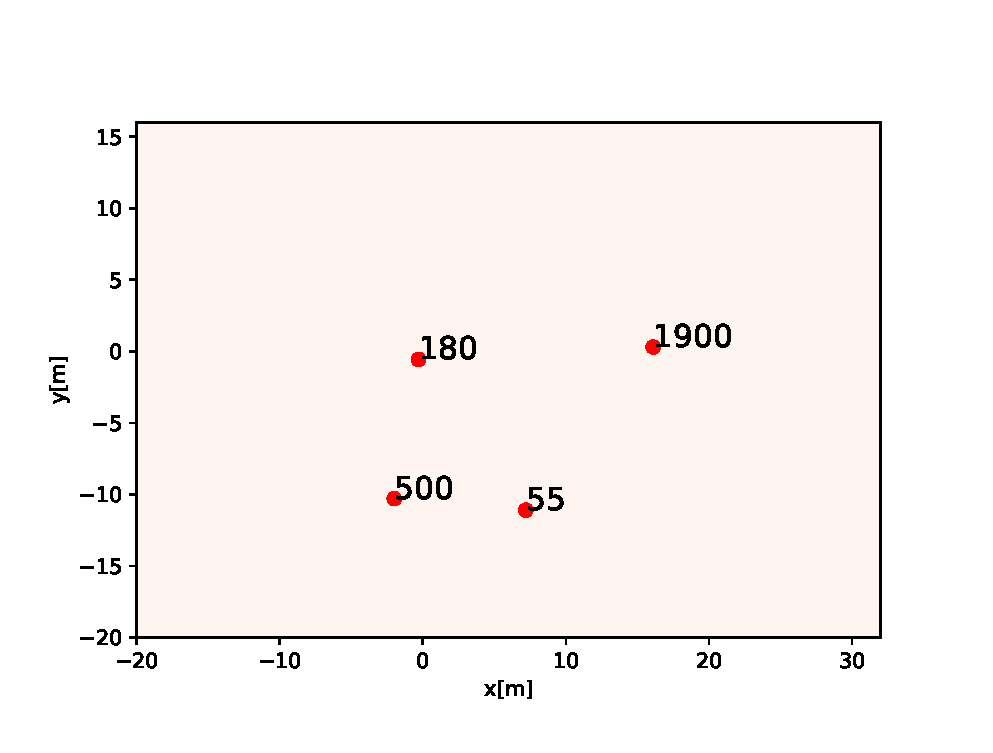
\includegraphics[width=0.5\textwidth]{./fig/photos/sources.eps}
    \label{fig:C}
  }
  \subfloat[MLEM estimate after 10 iterations] {
    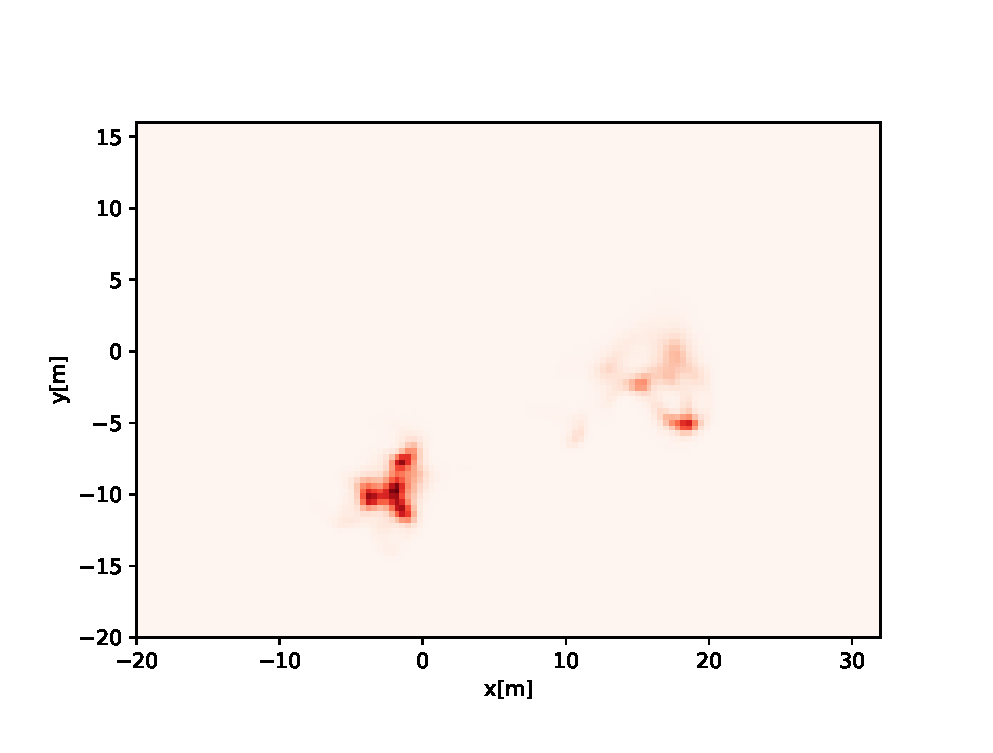
\includegraphics[width=0.5\textwidth]{./fig/photos/lambdas.eps}
    \label{fig:D}
  }
  \label{fig:A}
  \caption{Comparison of MLEM algorithm estimate and the ground truth.}
\end{figure}


\begin{figure}[!htb]
  \centering
  \subfloat[System matrix $\mathbf{T}$ summed over $\forall i$] {
    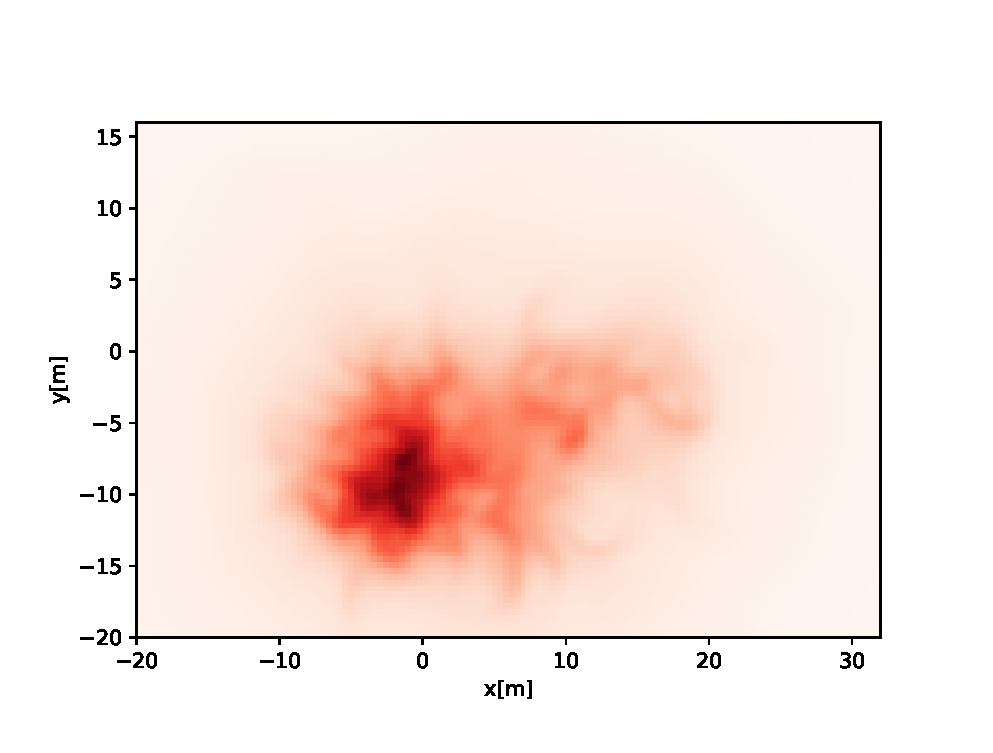
\includegraphics[width=0.5\textwidth]{./fig/photos/t.eps}
    \label{fig:E}
  }

  \subfloat[Sensitivity vector $\mathbf{s}$] {
    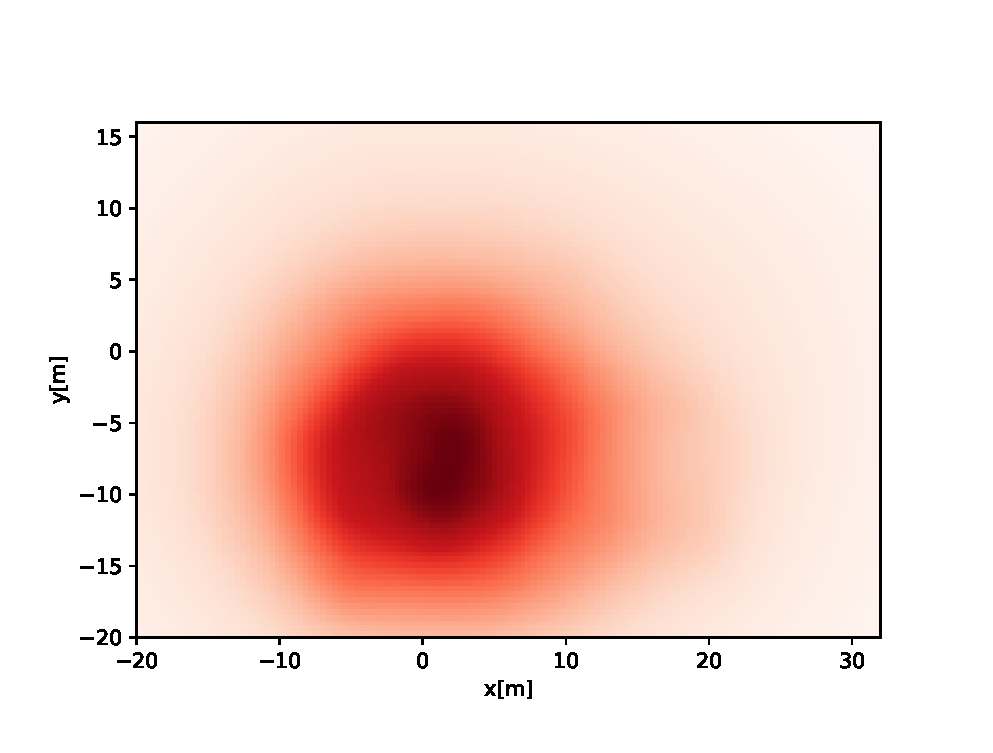
\includegraphics[width=0.5\textwidth]{./fig/photos/sensitivity.eps}
    \label{fig:F}
  }
  \label{fig:B}
  \caption{System matrix and sensitivity vector estimated during the experiment}

\end{figure}

\section{Discussion}
We can see that the algorithm precisely detected the 500 MBq source. Two smallest source were not recognised, probably due to low number of cones measured.
The 1900 MBg source was partially detected. 
In is important to note that the drones were flying mostly around the 500 MBg source and most of the measured cones originated from that source, as we can see in the sensitivity vector and system matrix in figure \ref{fig:B}.
This approach seems to be beneficial compared to naive back-projection of the cones to the map (without weighting with the sensitivity).



